\chapter{Introduction}
\vspace{-0.7em}
\minitoc
\begin{figure}[h]
    \centering
    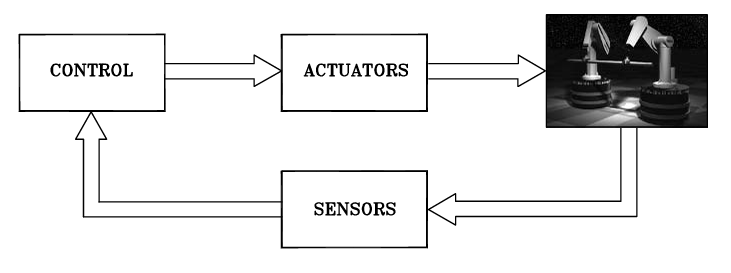
\includegraphics[scale=0.8]{img/robotic_system.png}
    \caption{Components of a robotic system}
\end{figure}
\vspace{-0.5cm}
\section{Robot: a possible definition}
\textit{What is robotics?} Before answering this question, it makes sense to rise up another question: \textbf{what is a robot?} Among all the available definitions the most suitable is the one provided by \textsf{Mike Brady}:
\begin{quotation}
    \colorbox{lightgray}{A robot realizes the \textit{intelligent} connection between \textbf{perception} and \textbf{action}.}
\end{quotation}
With reference to such a definition we can dissect it finding useful insights. A \textit{robotic system} is in the reality a complex system which is functionally represented by \textbf{multiple subsystems}. In particular you have a \textit{mechanical systems} which is made up of two apparatus: \textbf{locomotion apparatus} and a \textbf{manipulation apparatus} by which the robot itself can carry out the task. Both these subsystems are provided with an \textit{actuation system} which \textbf{animates} the mechanical part (this includes \textit{servomotors,drives} and \textit{transmissions})\footnote{
    It is quite clear that the \textbf{action} part is linked to the actuation system
}
The \textbf{perception} part rely on sensors which can acquire data about either the \underline{internal status} of the mechanical system (\textit{proprioceptive sensors}, eg. position transducers) or the \underline{external status} of the environments (they are called \textit{esteroceptive sensors}, eg. cameras).\\
The connection between the the actuation and sensing part is provided by a \textit{control system} which in an intelligent way can command the execution of some actions. It is remarkable that the control system exploits a mathematical model of the robot.\\
At this point, we can say that \textbf{Robotics} deals with
\begin{center}
    \normalsize
    \colorbox{lightgray}{\textbf{study} and \textbf{design} of robots.}
\end{center}
this is the reason why it results in an interdisciplinary subject involving \textit{mechanics, control, computers} and \textit{electronics}.\\
The term \textbf{robot} it is derived from the Slav term \textit{robota} (executive labor), and it appeared several years before any robot could be built!

\section{Robots classification}
Nowadays, robots can be used in different contexts according to which they are split in: 
\begin{itemize}
    \itemsep-0.2em
    \item \textsf{Industrial robots} they are used in the industrial field in order to perform several tasks such as soldering, moving part, cutting parts and so on; 
    \item \textsf{Humanoid and biometric robots} they are employed in order to interact with people or animal environments. Not rarely their mechanics is inspired by the real (natural) behaviour. 
    \item \textsf{Service robots} are used in contexts where the actions to be carried out are dangerous for human beings. For example: think about manipulating radioactive matter.
    \item \textsf{Exploration robots} are used, for example, in the field of space missions to study the atmosphere and the surface of Mars.
\end{itemize}

Another available classification of robots is the one based on the type of mechanical structure. Is the robot base moving or is it fixed? In the first case we are talking about \textbf{mobile robots} (humanoid/biometric, service and exploration robots often fall in this category), in the latter case we refer them with the term of \textbf{robot manipulators} (the great majority of industrial robots).

\subsection{Robot manipulator (Industrial robots)}
We anticipate here that a \textit{robot manipulator} is made up of a \underline{sequence of rigid bodies} (links) connected by means of articulations (\textit{joints}); the part of the manipulator that ensures mobility is the so-called \textbf{arm}, the part devoted to its agility (more technically, dexterity) is the \textbf{wrist} finally the part which perfors the action  is the \textbf{end-effector}. Several types of robot manipulators are obtained changing such components.

\begin{figure}
    \centering
    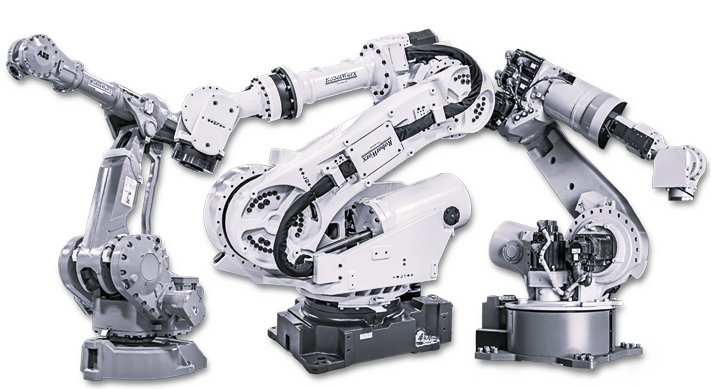
\includegraphics[scale=0.4]{img/3_Industrial_Robots.png}
    \caption{Examples of Industrial Robots}
\end{figure}

\subsection{Mobile robots}
The main feature here is the presence of a \textit{mobile base} which allows the robot to move into the environment it is placed. They are provided with a locomotion system that can be different (wheels, legs, wings...).



\section{Robot modeling, planning and control}
The totality of the tasks to be completed requires the execution of a \textit{specific motion prescribed to the robot}. The correct execution of the motion is entrusted to the control systems which should provide actuators with \textbf{command} consitstent with the desired motion (motion control), this -- in turn -- rely on an accurate analysis on the features of (jointly) mechanical structrure, actuators and sensors. The final aim of such an analysis is the derivation of a mathematical model describing the I/O relationship for the robot components (modeling component). Relevant topics in \textit{modeling, planning} and \textit{control} are briefly resumed in the following. 
\vspace{-0.3cm}
\subsection{Modelling}
Obtaining a model for a robot (industrial or mobile) concerns essentially in studying both the \textbf{kinematics} and \textbf{dynamics}. The former is the description of the robot motion without taking into account forces and torques which causes it. The latter describes forces and torques which generates the motion.\\
A further distinction is made between between \textit{kinematics} and \textit{differential kinematics} is made. In the first case we want to find a relationship between the joints and end-effector positions. In the second case we want to study the relationship between the joint and end-effector motion by means of velocity. A very useful tool in this case is the \textit{Jacobian} of the manipulator.\\
We conclude this discussion by saying that having a model for the robot is useful for the mechanical design of the structure, choice of actuators, determination of control strategies and for doing computer-based simulations.
\vspace{-0.3cm}
\subsection{Planning}
Every robot performs a task, for example for a manipulator we have the necessity to describe in some way the motion at the joints or at the end-effector. In material-handling task for example it is sufficient to decide an initial position and and end position (\textit{point-to-point} motion) in other situations we have to track a certain trajecotry (\textit{path motion}). In all these cases the task is the \textbf{trajectory planning} that is the determination of timing laws for relevant variables. For a mobile robot, such a task is even more complicate since it requires to take into account the constraints imposed by the wheels, legs, wings...
\vspace{-0.3cm}
\subsection{Control}
The generated trajectories constitutes the reference signal for the \textit{control system} of the mechanical structure. Techniques for controlling manipulators and mobile robots are very different how we will see this is due the presence or not of the interaction robot-environment and of the mobile base.

